%-----------------------------------------------------------------------------------------------------------------------------------------------%
%	The MIT License (MIT)
%
%	Copyright (c) 2015 Jan Küster
%
%	Permission is hereby granted, free of charge, to any person obtaining a copy
%	of this software and associated documentation files (the "Software"), to deal
%	in the Software without restriction, including without limitation the rights
%	to use, copy, modify, merge, publish, distribute, sublicense, and/or sell
%	copies of the Software, and to permit persons to whom the Software is
%	furnished to do so, subject to the following conditions:
%	
%	THE SOFTWARE IS PROVIDED "AS IS", WITHOUT WARRANTY OF ANY KIND, EXPRESS OR
%	IMPLIED, INCLUDING BUT NOT LIMITED TO THE WARRANTIES OF MERCHANTABILITY,
%	FITNESS FOR A PARTICULAR PURPOSE AND NONINFRINGEMENT. IN NO EVENT SHALL THE
%	AUTHORS OR COPYRIGHT HOLDERS BE LIABLE FOR ANY CLAIM, DAMAGES OR OTHER
%	LIABILITY, WHETHER IN AN ACTION OF CONTRACT, TORT OR OTHERWISE, ARISING FROM,
%	OUT OF OR IN CONNECTION WITH THE SOFTWARE OR THE USE OR OTHER DEALINGS IN
%	THE SOFTWARE.
%	
%
%-----------------------------------------------------------------------------------------------------------------------------------------------%


%============================================================================%
%
%	DOCUMENT DEFINITION
%
%============================================================================%

%we use article class because we want to fully customize the page and dont use a cv template
\documentclass[10pt,a4paper]{article}	


%----------------------------------------------------------------------------------------
%	ENCODING
%----------------------------------------------------------------------------------------

%we use utf8 since we want to build from any machine
\usepackage[utf8]{inputenc}		

%----------------------------------------------------------------------------------------
%	LOGIC
%----------------------------------------------------------------------------------------

% provides \isempty test
\usepackage{xifthen}

%----------------------------------------------------------------------------------------
%	FONT
%----------------------------------------------------------------------------------------

% some tex-live fonts - choose your own

%\usepackage[defaultsans]{droidsans}
%\usepackage[default]{comfortaa}
%\usepackage{cmbright}
\usepackage[default]{raleway}
%\usepackage{fetamont}
%\usepackage[default]{gillius}
%\usepackage[light,math]{iwona}
%\usepackage[thin]{roboto} 

% set font default
\renewcommand*\familydefault{\sfdefault} 	
\usepackage[T1]{fontenc}

% more font size definitions
\usepackage{moresize}		


%----------------------------------------------------------------------------------------
%	PAGE LAYOUT  DEFINITIONS
%----------------------------------------------------------------------------------------

%debug page outer frames
%\usepackage{showframe}			


%define page styles using geometry
\usepackage[a4paper]{geometry}		

% for example, change the margins to 2 inches all round
\geometry{top=1.75cm, bottom=-.6cm, left=1.5cm, right=1.5cm} 	

%use customized header
\usepackage{fancyhdr}				
\pagestyle{fancy}

%less space between header and content
\setlength{\headheight}{-5pt}		


%customize entries left, center and right
\lhead{}
\chead{ \small{César Sebastian Carrazana  $\cdot$ Lic. en Análisis de Sistemas $\cdot$  CABA, Argentina  $\cdot$  \textcolor{sectcol}{\textbf{cesarcarrazana@gmail.com}}  $\cdot$ +54 11 31081285}}
\rhead{}


%indentation is zero
\setlength{\parindent}{0mm}

%----------------------------------------------------------------------------------------
%	TABLE /ARRAY DEFINITIONS
%---------------------------------------------------------------------------------------- 

%for layouting tables
\usepackage{multicol}			
\usepackage{multirow}

%extended aligning of tabular cells
\usepackage{array}

\newcolumntype{x}[1]{%
>{\raggedleft\hspace{0pt}}p{#1}}%


%----------------------------------------------------------------------------------------
%	GRAPHICS DEFINITIONS
%---------------------------------------------------------------------------------------- 

%for header image
\usepackage{graphicx}

%for floating figures
\usepackage{wrapfig}
\usepackage{float}
%\floatstyle{boxed} 
%\restylefloat{figure}

%for drawing graphics		
\usepackage{tikz}				
\usetikzlibrary{shapes, backgrounds,mindmap, trees}


%----------------------------------------------------------------------------------------
%	Color DEFINITIONS
%---------------------------------------------------------------------------------------- 

\usepackage{color}

%accent color
\definecolor{sectcol}{RGB}{255,150,0}

%dark background color
\definecolor{bgcol}{RGB}{110,110,110}

%light background / accent color
\definecolor{softcol}{RGB}{225,225,225}


%============================================================================%
%
%
%	DEFINITIONS
%
%
%============================================================================%

%----------------------------------------------------------------------------------------
% 	HEADER
%----------------------------------------------------------------------------------------

% remove top header line
\renewcommand{\headrulewidth}{0pt} 

%remove botttom header line
\renewcommand{\footrulewidth}{0pt}	  	

%remove pagenum
\renewcommand{\thepage}{}	

%remove section num		
\renewcommand{\thesection}{}			

%----------------------------------------------------------------------------------------
% 	ARROW GRAPHICS in Tikz
%----------------------------------------------------------------------------------------

% a six pointed arrow poiting to the left
\newcommand{\tzlarrow}{(0,0) -- (0.2,0) -- (0.3,0.2) -- (0.2,0.4) -- (0,0.4) -- (0.1,0.2) -- cycle;}	

% include the left arrow into a tikz picture
% param1: fill color
%
\newcommand{\larrow}[1]
{\begin{tikzpicture}[scale=0.58]
	 \filldraw[fill=#1!100,draw=#1!100!black]  \tzlarrow
 \end{tikzpicture}
}

% a six pointed arrow poiting to the right
\newcommand{\tzrarrow}{ (0,0.2) -- (0.1,0) -- (0.3,0) -- (0.2,0.2) -- (0.3,0.4) -- (0.1,0.4) -- cycle;}

% include the right arrow into a tikz picture
% param1: fill color
%
\newcommand{\rarrow}
{
\begin{tikzpicture}[scale=0.7]
	\filldraw[fill=sectcol!100,draw=sectcol!100!black] \tzrarrow
 \end{tikzpicture}
}



%----------------------------------------------------------------------------------------
%	custom sections
%----------------------------------------------------------------------------------------

% create a coloured box with arrow and title as cv section headline
% param 1: section title
%
\newcommand{\cvsection}[1]
{
\colorbox{sectcol}{\mystrut \makebox[1\linewidth][l]{
\larrow{bgcol} \hspace{-8pt} \larrow{bgcol} \hspace{-8pt} \larrow{bgcol} \textcolor{white}{\textbf{#1}}\hspace{4pt}
}}\\
}

%create a coloured arrow with title as cv meta section section
% param 1: meta section title
%
\newcommand{\metasection}[2]
{
\begin{tabular*}{1\textwidth}{p{2.4cm} p{11cm}}
\larrow{bgcol}	\normalsize{\textcolor{sectcol}{#1}}&#2\\[12pt]
\end{tabular*}
}

%----------------------------------------------------------------------------------------
%	 CV EVENT
%----------------------------------------------------------------------------------------

% creates a stretched box as cv entry headline followed by two paragraphs about 
% the work you did
% param 1:	event time i.e. 2014 or 2011-2014 etc.
% param 2:	event name (what did you do?)
% param 3:	institution (where did you work / study)
% param 4:	what was your position
% param 5:	some words about your contributions
%
\newcommand{\cvevent}[5]
{
\vspace{8pt}
	\begin{tabular*}{1\textwidth}{p{2.3cm}  p{10.8cm} x{3.9cm}}
 \textcolor{bgcol}{#1}& \textbf{#2} & \vspace{2.5pt}\textcolor{sectcol}{#3}

	\end{tabular*}
\vspace{-12pt}
\textcolor{softcol}{\hrule}
\vspace{6pt}
	\begin{tabular*}{1\textwidth}{p{2.3cm} p{14.4cm}}
&		 \larrow{bgcol}  #4\\[3pt]
&		 \larrow{bgcol}  #5\\[6pt]
	\end{tabular*}

}

% creates a stretched box as 
\newcommand{\cveventmeta}[2]
{
	\mbox{\mystrut \hspace{87pt}\textit{#1}}\\
	#2
}

%----------------------------------------------------------------------------------------
% CUSTOM STRUT FOR EMPTY BOXES
%----------------------------------------- -----------------------------------------------
\newcommand{\mystrut}{\rule[-.3\baselineskip]{0pt}{\baselineskip}}

%----------------------------------------------------------------------------------------
% CUSTOM LOREM IPSUM
%----------------------------------------------------------------------------------------
\newcommand{\lorem}
{Lorem ipsum dolor sit amet, consectetur adipiscing elit. Donec a diam lectus.}



%============================================================================%
%
%
%
%	DOCUMENT CONTENT
%
%
%
%============================================================================%
\begin{document}


%use our custom fancy header definitions
\pagestyle{fancy}	


%---------------------------------------------------------------------------------------
%	TITLE HEADLINE
%----------------------------------------------------------------------------------------
\vspace{-20.55pt}

% use this for multiple words like working titles etc.
%\hspace{-0.25\linewidth}\colorbox{bgcol}{\makebox[1.5\linewidth][c]{\hspace{46pt}\HUGE{\textcolor{white}{\textsc{Jan Küster}} } \textcolor{sectcol}{\rule[-1mm]{1mm}{0.9cm}} \parbox[b]{5cm}{   \large{ \textcolor{white}{{IT Consultant}}}\\
% \large{ \textcolor{white}{{Resume}}}}
%}}

% use this for single words, e.g. CV or RESUME etc.
\hspace{-0.25\linewidth}\colorbox{bgcol}{\makebox[1.5\linewidth][c]{\HUGE{\textcolor{white}{\textsc{César Carrazana}} } \textcolor{sectcol}{\rule[-1mm]{1mm}{0.9cm}} \HUGE{\textcolor{white}{\textsc{Curriculum Vitae}} } }}


%----------------------------------------------------------------------------------------
%	HEADER IMAGE
%----------------------------------------------------------------------------------------

\begin{figure}[H]
\begin{flushright}
	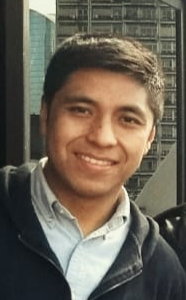
\includegraphics[clip,height=0.2\linewidth]{csc.jpg}	%trimming relative to image size!
\end{flushright}
\end{figure}

%---------------------------------------------------------------------------------------
%	QR CODE (optional)
%----------------------------------------------------------------------------------------
%\vspace{-136pt}
%\hspace{0.75\linewidth}
%\includegraphics[width=103pt]{qrcode}
%\normalsize
%\vspace{88pt}

%---------------------------------------------------------------------------------------
%	META SECTION
%----------------------------------------------------------------------------------------

\vspace{-114pt}

\metasection{Actual:}{Analista programador en TijeTravel}
\metasection{Campos:}{Desarrollo de software, Investigación}
\metasection{Preferencias:}{PHP, Symofny, MongoDB, Python, NodeJS, AngularJS, Docker}
\metasection{Actividades:}{Triatleta amateur}

\vspace{6pt}

%---------------------------------------------------------------------------------------
%	SUMMARAY (optional)
%----------------------------------------------------------------------------------------

%\cvsection{Summary}\\
%Digital media graduate with four years project experience in the field of technology based assessment. Specialized in development of test-scenario engines and innovative, rich media item formats. Master studies focused on teams from different disciplines and cultural backgrounds on solutions for complex problems.  Prior knowledge has been collected in he field of usability / accessibility during bachelor studies.\\

%============================================================================%
%
%	CV SECTIONS AND EVENTS (MAIN CONTENT)
%
%============================================================================%

%---------------------------------------------------------------------------------------
%	EXPERIENCE
%----------------------------------------------------------------------------------------
\cvsection{Experiencia}


\cvevent{2017 - Act}{Analista programador}{TijeTravel}{Captura y Análisis de requisitos}{Desarrollo e Implementación de soluciones}

\cvevent{2015 - Act}{Programador}{Freelance}{Desarrollo de software contable}{Desarrollo backend, procesos a bajo nivel en Linux, y funcionalidades especificas Android}

\cvevent{2013 - 2016}{Analista programador}{Min. de Rel. Ext. y Culto}{Relevamiento de funcionalidades, analisis de requerimientos, diseño y definicion de procesos, testing}{Herramientas de desarrollo: CakePHP, Symfony2, Javascript(Jquery, JSON, Ajax), CSS, HTML.}

\cvevent{2012 - 2013}{Analista Programador}{TijeTravel}{Certificación de procesos de reservas de Vuelos y Extreme Search AMADEUS Web Services.}{Implementación de pago electrónico y pasarela de pagos, planas y encriptadas.}

\cvevent{2010 - 2012}{Analista Funcional Técnico}{G.M.S. S.A.}{Relevamiento de funcionalidad con cliente y documentación en Casos de Uso, posterior monitoreo de tareas.}{Reportes e integración de herramientas IT como ExtJS, WebServices .Net, SqlServer, Sencha Touch.}

\cvevent{2010 - 2011}{Analista Programador}{eSalud Americas}{Analista Programador (Desarrollo e integración de soluciones TIC aplicadas al sector salud)}{Desarrollo de aplicaciones orientadas al monitoreo de pacientes remotos. Herramientas ExtJs, PHP, Javascript, HTML, Flot, Redmine.}

\cvevent{2010 - 2010}{Programador}{NexoDigital}{Desarrollador PHP, Part time, Salta}{Desarrollo de herramientas internas. PHP, JavaScript, HTML, CSS, MySql}

\cvevent{2010 - 2010}{Programador}{Metasitios}{Desarrollador Jr. PHP Symfony, Part time, Salta.
}{Desarrollo de plataforma de sorteos web para clientes de España.}

\hfill \break

%---------------------------------------------------------------------------------------
%	EDUCATION SECTION
%--------------------------------------------------------------------------------------
\cvsection{Educación}

\cvevent{2003 – 2010}{Licenciatura en Análisis de Sistemas}{Universidad Nacional de Salta}{Título de
Grado.}{Licenciatura en Analisis de Sistemas}

\cvevent{2003 – 2007}{Computador Universitario}{Universidad Nacional de Salta}{Título intermedio de la carrera de Licenciatura en Análisis de Sistemas.}{Programador Universitario}

\cvevent{1998 – 2002}{Título secundario}{Escuela Normal Sup. Rep. de Bolivia}{Bachiller Nacional, Jujuy-Humahuaca}{Orientacion Bachiller}

%---------------------------------------------------------------------------------------
%	CUSROS
%--------------------------------------------------------------------------------------
\cvsection{Cursos, Jornadas y Congresos}

\metasection{2019}{Curso de Arquitectura de Software - EscuelaIT - España}
\metasection{2016}{Curso de Patrones de Diseño - EscuelaIT - España}
\metasection{2016}{Curso Ingles Nivel 2 Modulo 1 Aprobado - Ministerio de Relaciones Exteriores y Culto}
\metasection{2015}{Curso Ingles Nivel 1 Modulo 2 Aprobado - Ministerio de Relaciones Exteriores y Culto}
\metasection{2015}{Curso Ingles Nivel 1 Modulo 1 Aprobado - Ministerio de Relaciones Exteriores y Culto}
\metasection{2015}{Curso de Android Developer- Educación IT }
\metasection{2010}{Curso de Desarrollo Web en Symfony - Empresa Metasitios}
\metasection{2010}{Certificación Java Programming - Fundación Pallay}
\metasection{2009}{Elementos de la Seguridad Informática - COPAIPA y Universidad Católica de Salta}
\metasection{2008}{Curso de Administración de Bases de Datos Oracle - 72hs con examen final. Universidad Nacional de Jujuy}
\metasection{2007}{Participación XXX Reunión de trabajos de la Asociación Argentina de Energía Renovables (ASADES) como integrante y expositor del proyecto: Adquisición de Datos y Monitoreo (DAMA). Universidad Nacional de San Luis }
\metasection{2006}{I Jornadas de Software Libre. Universidad Nacional de Salta}
\metasection{2005}{Seguridad en Sistemas Informáticos. Universidad Nacional de Salta}

%---------------------------------------------------------------------------------------
%	Otros datos de Interés
%--------------------------------------------------------------------------------------
\cvsection{Otros datos de Interés}

\metasection{2015}{Reconocimiento por desarrollo de Sistema de Elecciones en el Exterior - CT DIRFE010031 2015 - ELECCIONES NACIONALES 2015: INFORMACION DE INTERES Y AGRADECIMIENTO - Ministerio de Relaciones Exteriores y Culto}
\metasection{2014}{Felicitaciones por desarrollo de herramienta de Reporte de Incidentes Mundial Brasil 2014 - Ministerio de Relaciones Exteriores y Culto}
\metasection{2009}{Beca Contro + F para la realización del Curso de Java Programming Intermedio}
\metasection{2008-2009}{Integrante del Pabellón de Abanderados de la Facultad de Ciencias Exactas}
\metasection{2006-2007}{Participación en el grupo de trabajo del Proyecto 1178 del CIUNSa, en el desarrollo de una herramienta software Java para el Telemonitoreo y control via web de Sistemas de Adquisición de datos basados en Módulos NuDAM, ADAM, PIC}
\metasection{2009}{Beca TICs de 5to año}
\metasection{2007}{Beca Económica del Programa Nacional de Becas Universitarias (PNBU)}
\metasection{2003-2004}{Beca Económica de la Universidad Nacional de Salta}

%-------------------------------------------------------------------------------------------------
%	ARTIFICIAL FOOTER (fancy footer cannot exceed linewidth) 
%--------------------------------------------------------------------------------------------------

\null
\vspace*{\fill}
\hspace{-0.25\linewidth}\colorbox{bgcol}{\makebox[1.5\linewidth][c]{\mystrut \small \textcolor{white}{cesarcarrazana@gmail.com} $\cdot$ \textcolor{white}{https://www.linkedin.com/in/ccarrazana/}}}




%============================================================================%
%
%
%
%	DOCUMENT END
%
%
%
%============================================================================%
\end{document}
